\subsection{Double Integrals over Rectangles}

Rectangle $R = [a,b]\times[c,d]$.

\begin{center}
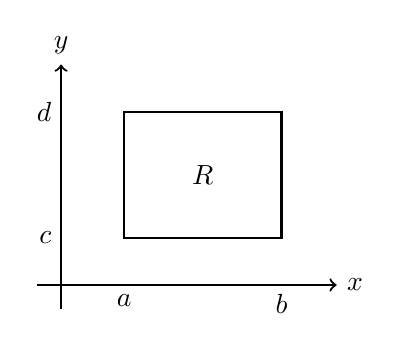
\begin{tikzpicture}
    \draw[thick,->] (-0.3,0) -- (3.5,0) node[right]{$x$};
    \draw[thick,->] (0,-0.3) -- (0,2.8) node[above]{$y$};
    \draw[thick] (0.8,0.6) rectangle (2.8,2.2);
    \node at (1.8,1.4) {$R$};
    \node[below] at (0.8,0) {$a$};
    \node[below] at (2.8,0) {$b$};
    \node[left] at (0,0.6) {$c$};
    \node[left] at (0,2.2) {$d$};
\end{tikzpicture}
\end{center}

\begin{center}
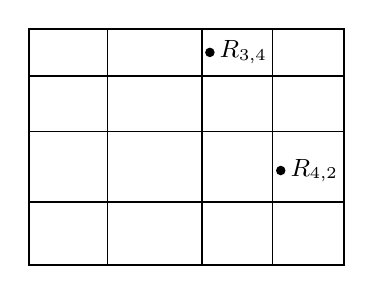
\begin{tikzpicture}
    % outer rectangle
    \draw[thick] (0,0) rectangle (4,3);
    % vertical grid lines
    \draw (1,0) -- (1,3);
    \draw (2.2,0) -- (2.2,3);
    \draw (3.1,0) -- (3.1,3);
    % horizontal grid lines
    \draw (0,0.8) -- (4,0.8);
    \draw (0,1.7) -- (4,1.7);
    \draw (0,2.4) -- (4,2.4);
    % sample points
    \filldraw (2.3,2.7) circle (1.5pt) node[right]{\small$R_{3,4}$};
    \filldraw (3.2,1.2) circle (1.5pt) node[right]{\small$R_{4,2}$};
\end{tikzpicture}
\end{center}

Subdivide $R$ into sub-rectangles with widths $\Delta x_i$, $\Delta y_j$.
Choose sample points $P_{ij} = (x_{ij},\, y_{ij})$.
Let $M = \max\{\Delta x_i,\, \Delta y_j\}$.

\begin{definition}{Double Integral}{double-int}
\[
    \iint_R f(x,y)\dd{A}
    := \lim_{M\to 0}\sum_{i=1}^{m}\sum_{j=1}^{n} f(P_{ij})\,\Delta x_i\,\Delta y_j
\]
\end{definition}

\begin{theorem}{}{continuous-integrable}
If $f$ is continuous on $R$, then $f$ is integrable (i.e.\ the double integral exists).
\end{theorem}

Evaluation of $\iint_R f\dd{A}$ by definition is usually difficult.

\textbf{Estimation:} $\displaystyle\sum\sum(\text{midpoint value}\times\text{area})$.

\begin{definition}{Average Value}{avg-value}
\[
    \text{average of } f(x,y) \text{ on } R
    = \frac{\iint_R f\dd{A}}{\operatorname{Area}(R)}
\]
\end{definition}

\subsubsection{Iterated Integrals}

\[
    \iint_R f\dd{A}
    \;\longrightarrow\;
    \int\!\!\int f\dd{x}\dd{y}
    \quad\text{(nested single-variable integrals)}
\]

For fixed $x^{*}\in[a,b]$, define
$\displaystyle A(x^{*}) = \int_c^d f(x^{*},y)\dd{y}$.

\begin{example}
$f(x,y) = xy^3$, \; $R = [1,3]\times[3,7]$.
For $x^{*}\in[1,3]$:
\[
    A(x^{*}) = \int_3^7 x^{*}\,y^3\dd{y}
    = \frac{x^{*}}{4}(7^4 - 3^4)
\]
\end{example}

\[
    \iint_R f(x,y)\dd{A} = \int_a^b A(x)\dd{x}
\]

\begin{theorem}{Fubini's Theorem}{fubini}
Suppose $f$ is continuous on $R = [a,b]\times[c,d]$. Then
\[
    \iint_R f(x,y)\dd{A}
    = \int_a^b\!\left(\int_c^d f(x,y)\dd{y}\right)\dd{x}
    = \int_c^d\!\left(\int_a^b f(x,y)\dd{x}\right)\dd{y}
\]
\end{theorem}

\begin{example}
$f(x,y) = x + y^2$. Compute $\displaystyle\int_0^1\!\int_2^3 f\dd{x}\dd{y}$.
\begin{align*}
    \int_0^1\!\int_2^3 (x+y^2)\dd{x}\dd{y}
    &= \int_0^1 \left[\frac{1}{2}x^2 + xy\right]_{x=2}^{3}\dd{y} \\
    &= \int_0^1 \left(\tfrac{5}{2} + y^2\right)\dd{y} \\[4pt]
    &= \left[\frac{5}{2}y + \frac{1}{3}y^3\right]_0^1
    = \frac{17}{6}
\end{align*}
\end{example}

\begin{example}
$\displaystyle\int_0^4\!\int_0^9 \sqrt{x+4y}\dd{x}\dd{y}$.
\begin{align*}
    &= \int_0^4 \left[\frac{2}{3}(x+4y)^{3/2}\right]_{x=0}^{9}\dd{y} \\
    &= \frac{2}{3}\int_0^4 (9+4y)^{3/2} - 8y^{3/2}\dd{y} \\
    &= \frac{2}{3}\left[\frac{1}{10}(9+4y)^{5/2}
      - \frac{16}{5}y^{5/2}\right]_0^4
    = \cdots
\end{align*}
\end{example}

\begin{example}
$\displaystyle\iint_R xe^{-xy}\dd{A}$, \; $R=[0,1]\times[0,2]$.

Integrate $y$ first since it is easier:
\begin{align*}
    \int_0^1\!\int_0^2 xe^{-xy}\dd{y}\dd{x}
    &= \int_0^1 \left[-e^{-xy}\right]_{y=0}^{2}\dd{x} \\
    &= \int_0^1 \left(1-e^{-2x}\right)\dd{x} \\
    &= \left[x+\tfrac{1}{2}e^{-2x}\right]_0^1
    = \tfrac{1}{2}(e^{-2}+1)
\end{align*}
\end{example}

\subsubsection{Analogue of the Fundamental Theorem of Calculus}

Suppose $\dfrac{\partial^{2}F}{\partial x\,\partial y}=f(x,y)$ is continuous on
$R=[a,b]\times[c,d]$. Then:
\begin{align*}
    \iint_R f\dd{A}
    &= \int_a^b\!\int_c^d \frac{\partial^{2}F}{\partial x\,\partial y}\dd{y}\dd{x} \\
    &= \int_a^b \left[\pd{F}{x}\right]_{y=c}^{y=d}\dd{x} \\
    &= \int_a^b \left[\pd{F}{x}(x,d)-\pd{F}{x}(x,c)\right]\dd{x} \\
    &= F(b,d) - F(a,d) - F(b,c) + F(a,c)
\end{align*}

\begin{center}
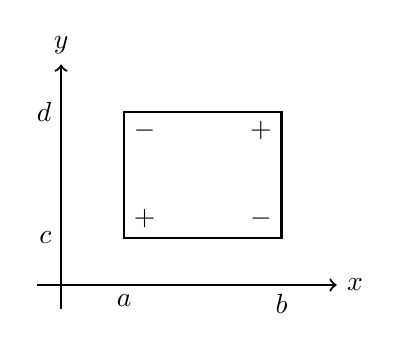
\begin{tikzpicture}
    \draw[thick,->] (-0.3,0) -- (3.5,0) node[right]{$x$};
    \draw[thick,->] (0,-0.3) -- (0,2.8) node[above]{$y$};
    \draw[thick] (0.8,0.6) rectangle (2.8,2.2);
    \node[below] at (0.8,0) {$a$};
    \node[below] at (2.8,0) {$b$};
    \node[left] at (0,0.6) {$c$};
    \node[left] at (0,2.2) {$d$};
    \node at (0.8,0.6) [above right] {$+$};
    \node at (2.8,0.6) [above left] {$-$};
    \node at (0.8,2.2) [below right] {$-$};
    \node at (2.8,2.2) [below left] {$+$};
\end{tikzpicture}
\end{center}

\subsection{Double Integrals over General Regions}

Suppose $D$ is a bounded region.
Extend $D$ to a rectangle $R\supseteq D$ and define
\[
    \tilde{f}(x,y)
    = \begin{cases} f(x,y) & (x,y)\in D \\ 0 & (x,y)\notin D \end{cases}
\]
Then $\displaystyle\iint_D f\dd{A} = \iint_R \tilde{f}\dd{A}$.

\subsubsection{Type I}

$x\in[a,b]$, \; $y\in[g_1(x),\, g_2(x)]$.

\begin{center}
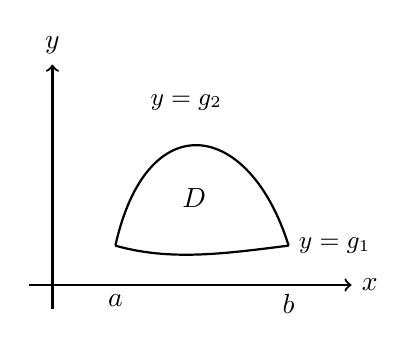
\begin{tikzpicture}
    \draw[thick,->] (-0.3,0) -- (3.8,0) node[right]{$x$};
    \draw[thick,->] (0,-0.3) -- (0,2.8) node[above]{$y$};
    \draw[thick] (0.8,0.5) .. controls (1.5,0.3) and (2.2,0.4) .. (3.0,0.5)
        node[right]{\small$y=g_1$};
    \draw[thick] (0.8,0.5) .. controls (1.2,2.3) and (2.5,2.1) .. (3.0,0.5);
    \node[above] at (1.7,2.1) {\small$y=g_2$};
    \node at (1.8,1.1) {$D$};
    \node[below] at (0.8,0) {$a$};
    \node[below] at (3.0,0) {$b$};
\end{tikzpicture}
\end{center}

\[
    \iint_D f\dd{A}
    = \int_a^b\!\int_{g_1(x)}^{g_2(x)} f\dd{y}\dd{x}
\]

\begin{example}
$D$: quarter disk, $x\in[0,1]$, $y\in[0,\sqrt{1-x^2}]$.

\begin{center}
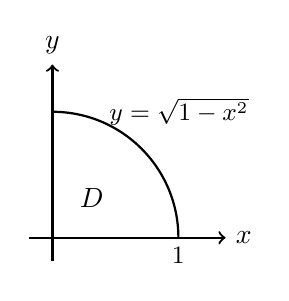
\begin{tikzpicture}
    \draw[thick,->] (-0.3,0) -- (2.2,0) node[right]{$x$};
    \draw[thick,->] (0,-0.3) -- (0,2.2) node[above]{$y$};
    \draw[thick] (1.6,0) arc[start angle=0, end angle=90, radius=1.6];
    \node[above right] at (0.6,1.3) {\small$y=\sqrt{1-x^2}$};
    \node at (0.5,0.5) {$D$};
    \node[below] at (1.6,0) {\small$1$};
\end{tikzpicture}
\end{center}

\begin{align*}
    \iint_D xy\dd{A}
    &= \int_0^1\!\int_0^{\sqrt{1-x^2}} xy\dd{y}\dd{x} \\
    &= \int_0^1 \left[\tfrac{1}{2}xy^2\right]_{y=0}^{\sqrt{1-x^2}}\dd{x} \\
    &= \int_0^1 \tfrac{1}{2}x(1-x^2)\dd{x}
    = \frac{1}{8}
\end{align*}
\end{example}

\subsubsection{Type II}

$y\in[c,d]$, \; $x\in[h_1(y),\, h_2(y)]$.

\begin{center}
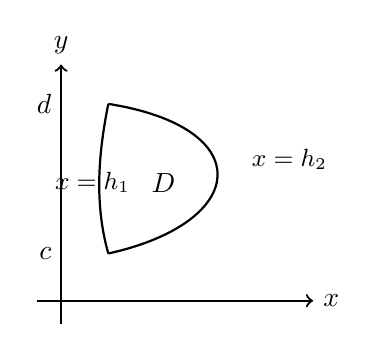
\begin{tikzpicture}
    \draw[thick,->] (-0.3,0) -- (3.2,0) node[right]{$x$};
    \draw[thick,->] (0,-0.3) -- (0,3.0) node[above]{$y$};
    \draw[thick] (0.6,0.6) .. controls (0.4,1.3) and (0.5,2.0) .. (0.6,2.5);
    \draw[thick] (0.6,0.6) .. controls (2.4,1.0) and (2.5,2.2) .. (0.6,2.5);
    \node[right] at (-0.2,1.5) {\small$x=h_1$};
    \node[right] at (2.3,1.8) {\small$x=h_2$};
    \node at (1.3,1.5) {$D$};
    \node[left] at (0,0.6) {$c$};
    \node[left] at (0,2.5) {$d$};
\end{tikzpicture}
\end{center}

\[
    \iint_D f\dd{A}
    = \int_c^d\!\int_{h_1(y)}^{h_2(y)} f\dd{x}\dd{y}
\]

\begin{example}[Volume of a Sphere]
$x^2+y^2+z^2=R^2$.
The height function is $h(x,y)=2z=2\sqrt{R^2-x^2-y^2}$.
\[
    \text{Volume} = \iint_D h\dd{A},
    \qquad D\colon x^2+y^2\le R^2
\]

\begin{center}
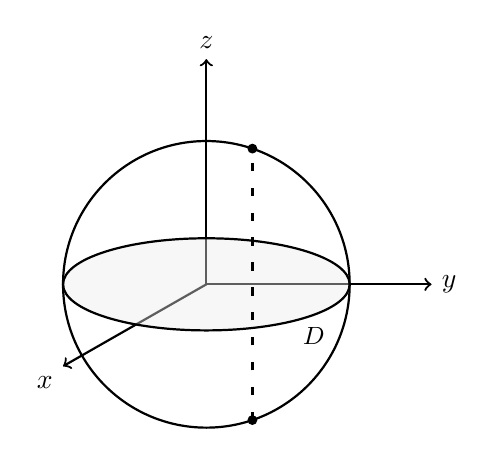
\begin{tikzpicture}[scale=1.3]
    % axes
    \draw[thick,->] (0,0) -- (-1.4,-0.8) node[below left]{$x$};
    \draw[thick,->] (0,0) -- (2.2,0) node[right]{$y$};
    \draw[thick,->] (0,0) -- (0,2.2) node[above]{$z$};
    % disk D on the xy-plane (equator plane) — filled for "plane" look
    \fill[gray!15, opacity=0.4] (0,0) ellipse (1.4 and 0.45);
    \draw[thick] (0,0) ellipse (1.4 and 0.45);
    \node at (1.05,-0.5) {\small$D$};
    % sphere centred at origin; equator coincides with disk
    \draw[thick] (0,0) circle (1.4);
    % vertical line touching top and bottom
    \draw[thick, loosely dashed] (0.45,-1.326) -- (0.45,1.326);
    \filldraw (0.45,-1.326) circle (1.2pt);
    \filldraw (0.45,1.326) circle (1.2pt);
\end{tikzpicture}
\end{center}

Type I: $x\in[-R,R]$, $y\in[-\sqrt{R^2-x^2},\,\sqrt{R^2-x^2}]$.
\[
    \text{Volume}
    = \int_{-R}^{R}\!\int_{-\sqrt{R^2-x^2}}^{\sqrt{R^2-x^2}}
      2\sqrt{R^2-x^2-y^2}\dd{y}\dd{x}
\]
By evenness:
\[
    = 4\int_0^{R}\!\int_0^{\sqrt{R^2-x^2}}
      2\sqrt{R^2-x^2-y^2}\dd{y}\dd{x}
    = \cdots
    = \frac{4}{3}\pi R^3
\]
Substitution: $y=\sqrt{R^2-x^2}\sin\theta$,
$\dd{y}=\sqrt{R^2-x^2}\cos\theta\dd{\theta}$.
\end{example}

\begin{example}[Fubini's Theorem — Switching Order of Integration]
Compute $\displaystyle\int_0^1\!\left(\int_{x^2}^{1}\sqrt{y}\sin y\dd{y}\right)\dd{x}$.

The inner integral is difficult to evaluate directly, so we use Fubini's theorem (Theorem~\ref{thm:fubini}) to switch the order of integration.

\textbf{1. Describe the domain $D$:}
$x\in[0,1]$, \; $y\in[x^2,\,1]$ \quad (Type I).

\begin{center}
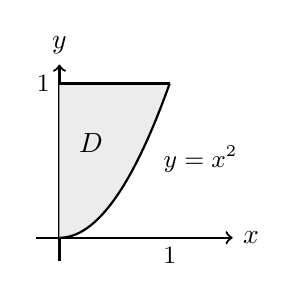
\begin{tikzpicture}
    \draw[thick,->] (-0.3,0) -- (2.2,0) node[right]{$x$};
    \draw[thick,->] (0,-0.3) -- (0,2.2) node[above]{$y$};
    \fill[gray!15] (0,0) parabola (1.4,1.96) -- (0,1.96) -- cycle;
    \draw[thick, domain=0:1.4, samples=50] plot (\x, {\x*\x});
    \draw[thick] (0,1.96) -- (1.4,1.96);
    \node at (0.4,1.2) {$D$};
    \node[below] at (1.4,0) {\small$1$};
    \node[left] at (0,1.96) {\small$1$};
    \node[right] at (1.2,1.0) {\small$y=x^2$};
\end{tikzpicture}
\end{center}

\textbf{2. Rewrite as Type II:}
$y\in[0,1]$, \; $x\in[0,\,\sqrt{y}]$.

\textbf{3. Evaluate:}
\begin{align*}
    \int_0^1\!\int_0^{\sqrt{y}}\sqrt{y}\sin y\dd{x}\dd{y}
    &= \int_0^1 \bigl[\sqrt{y}\sin y\cdot x\bigr]_{x=0}^{\sqrt{y}}\dd{y}
    = \int_0^1 y\sin y\dd{y}
\end{align*}
Integration by parts ($u=y$, $\dd{v}=\sin y\dd{y}$):
\begin{align*}
    &= \bigl[-y\cos y\bigr]_0^1 + \int_0^1\cos y\dd{y}
    = -\cos 1 + \bigl[\sin y\bigr]_0^1
    = \sin 1 - \cos 1
\end{align*}
\end{example}

\subsubsection{Properties of Double Integrals}

\begin{enumerate}
    \item $\displaystyle\iint_D 1\dd{A} = \operatorname{Area}(D)$
    \item $f(x,y)\le g(x,y)$ for all $(x,y)\in D
          \;\Longrightarrow\;
          \displaystyle\iint_D f\dd{A}\le\iint_D g\dd{A}$
    \item $m\le f\le M$ on $D
          \;\Longrightarrow\;
          m\cdot\operatorname{Area}(D)
          \le\displaystyle\iint_D f\dd{A}
          \le M\cdot\operatorname{Area}(D)$
\end{enumerate}

\begin{example}[Estimation]
Estimate $\displaystyle\iint_D\cos(x^2 y^2)\dd{A}$
where $D=\bigl[0,\frac{\pi}{4}\bigr]\times\bigl[0,\frac{\pi}{4}\bigr]$.

\begin{center}
\begin{tikzpicture}
    \draw[thick,->] (-0.3,0) -- (2.2,0) node[right]{$x$};
    \draw[thick,->] (0,-0.3) -- (0,2.2) node[above]{$y$};
    \draw[thick] (0,0) rectangle (1.5,1.5);
    \node[below] at (1.5,0) {\small$\frac{\pi}{4}$};
    \node[left] at (0,1.5) {\small$\frac{\pi}{4}$};
\end{tikzpicture}
\end{center}

$M = \max(f\text{ on }D) = 1$, \;
$m = \min(f\text{ on }D) = \cos\!\left(\dfrac{\pi^4}{256}\right)$.

By property 3:
\[
    \cos\!\left(\frac{\pi^4}{256}\right)\cdot\frac{\pi^2}{16}
    \;\le\; \iint_D\cos(x^2 y^2)\dd{A}
    \;\le\; \frac{\pi^2}{16}
\]
\end{example}

\subsection{Double Integrals in Polar Coordinates}

Compute $\iint_D f\dd{A}$ when:
\begin{enumerate}
    \item $D$ is nice in polar coordinates
    \item $f$ is nice in polar coordinates,
          e.g.\ $f(x,y)=x^2+y^2=r^2$
\end{enumerate}

In normal coordinates $\dd{A}=\dd{x}\dd{y}$;
in polar coordinates $\dd{A}=r\dd{r}\dd{\theta}$.

\begin{center}
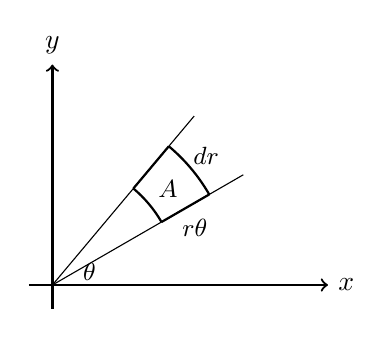
\begin{tikzpicture}
    \draw[thick,->] (-0.3,0) -- (3.5,0) node[right]{$x$};
    \draw[thick,->] (0,-0.3) -- (0,2.8) node[above]{$y$};
    % wedge element
    \draw (0,0) -- (50:2.8);
    \draw (0,0) -- (30:2.8);
    \draw[thick] (30:1.6) arc[start angle=30, end angle=50, radius=1.6];
    \draw[thick] (30:2.3) arc[start angle=30, end angle=50, radius=2.3];
    \draw[thick] (30:1.6) -- (30:2.3);
    \draw[thick] (50:1.6) -- (50:2.3);
    \node at (40:2.55) {\small$dr$};
    \node at (22:1.95) {\small$r\dd{\theta}$};
    \node[below right] at (50:1.9) {\small$\dd{A}$};
    \node at (20:0.5) {\small$\dd{\theta}$};
\end{tikzpicture}
\end{center}

\begin{theorem}{Change to Polar Coordinates}{polar-change}
\[
    \iint_D f\dd{A}
    = \int_\alpha^\beta\!\int_a^b
      f(r\cos\theta,\,r\sin\theta)\;r\dd{r}\dd{\theta}
\]
\end{theorem}

\begin{example}[Volume under a Paraboloid]
Find the volume under $z=4-x^2-y^2$ above $z=0$.

\begin{center}
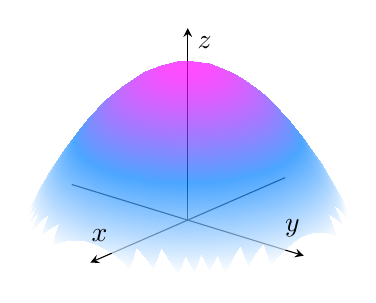
\begin{tikzpicture}
    \begin{axis}[
        view={130}{30}, width=7cm, height=6cm,
        xlabel=$x$, ylabel=$y$, zlabel=$z$,
        domain=-2:2, y domain=-2:2,
        samples=30, colormap/cool,
        axis lines=center, ticks=none,
        zmin=0, zmax=5,
    ]
    \addplot3[surf, opacity=0.7, shader=interp,
        restrict z to domain=0:4]{4-x^2-y^2};
    \end{axis}
\end{tikzpicture}
\end{center}

$D$ in polar: $0\le r\le 2$, $0\le\theta\le 2\pi$.
\begin{align*}
    \text{Volume}
    &= \int_0^{2\pi}\!\int_0^{2}(4-r^2)\,r\dd{r}\dd{\theta} \\
    &= \int_0^{2\pi}\dd{\theta}\;\int_0^{2}(4r-r^3)\dd{r}
    \quad\text{(separable)} \\
    &= 2\pi\left[2r^2-\tfrac{r^4}{4}\right]_0^2
    = 2\pi\cdot 4 = 8\pi
\end{align*}
\end{example}

\begin{example}[Quarter Ring]
$\displaystyle\iint_D(x+y)\dd{A}$, \;
$D$: quarter ring, $4\le x^2+y^2\le 16$, $0\le\theta\le\pi/2$.

\begin{center}
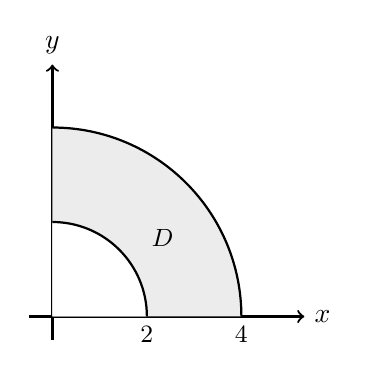
\begin{tikzpicture}
    \draw[thick,->] (-0.3,0) -- (3.2,0) node[right]{$x$};
    \draw[thick,->] (0,-0.3) -- (0,3.2) node[above]{$y$};
    \fill[gray!15] (0,0) -- (2.4,0) arc[start angle=0, end angle=90, radius=2.4]
        -- cycle;
    \fill[white] (0,0) -- (1.2,0) arc[start angle=0, end angle=90, radius=1.2]
        -- cycle;
    \draw[thick] (1.2,0) arc[start angle=0, end angle=90, radius=1.2];
    \draw[thick] (2.4,0) arc[start angle=0, end angle=90, radius=2.4];
    \node at (1.4,1.0) {\small$D$};
    \node[below] at (1.2,0) {\small$2$};
    \node[below] at (2.4,0) {\small$4$};
\end{tikzpicture}
\end{center}

\begin{align*}
    &= \int_0^{\pi/2}\!\int_2^4
       (r\cos\theta+r\sin\theta)\,r\dd{r}\dd{\theta} \\
    &= \int_0^{\pi/2}(\cos\theta+\sin\theta)\dd{\theta}
       \;\int_2^4 r^2\dd{r}
       \quad\text{(separable)} \\
    &= (2)\!\left(\tfrac{1}{3}(4^3-2^3)\right)
    = \frac{112}{3}
\end{align*}
\end{example}

\subsubsection{General Polar Regions}

Generalization of Type I/II to polar coordinates:

\begin{center}
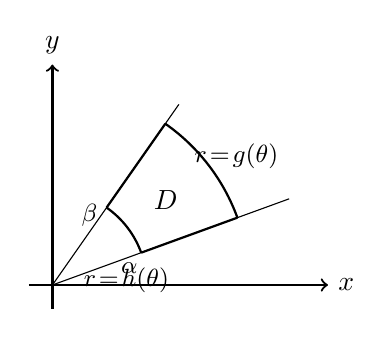
\begin{tikzpicture}
    \draw[thick,->] (-0.3,0) -- (3.5,0) node[right]{$x$};
    \draw[thick,->] (0,-0.3) -- (0,2.8) node[above]{$y$};
    \draw (0,0) -- (20:3.2);
    \draw (0,0) -- (55:2.8);
    \draw[thick] (20:1.2) arc[start angle=20, end angle=55, radius=1.2];
    \draw[thick] (20:2.5) arc[start angle=20, end angle=55, radius=2.5];
    \draw[thick] (20:1.2) -- (20:2.5);
    \draw[thick] (55:1.2) -- (55:2.5);
    \node at (37:1.8) {$D$};
    \node[below] at (20:1.0) {\small$r\!=\!h(\theta)$};
    \node[above] at (30:2.7) {\small$r\!=\!g(\theta)$};
    \node at (12:1.0) {\small$\alpha$};
    \node at (62:1.0) {\small$\beta$};
\end{tikzpicture}
\end{center}

\[
    \iint_D f\dd{A}
    = \int_\alpha^\beta\!\int_{h(\theta)}^{g(\theta)} f\;r\dd{r}\dd{\theta}
\]

\begin{example}[Area of a Polar Curve]
Find the area enclosed by $r^2=4-3\cos 5\theta$.

$D\colon 0\le\theta\le 2\pi$, \; $0\le r\le\sqrt{4-3\cos 5\theta}$.
\begin{align*}
    \text{Area}
    &= \int_0^{2\pi}\!\int_0^{\sqrt{4-3\cos 5\theta}} r\dd{r}\dd{\theta}
    = \int_0^{2\pi}\tfrac{1}{2}(4-3\cos 5\theta)\dd{\theta}
    = 4\pi
\end{align*}
\end{example}

\begin{example}[Cartesian to Polar]
Evaluate $\displaystyle\int_0^{2}\!\int_x^{\sqrt{3}\,x} y\dd{y}\dd{x}$
using polar coordinates.

\begin{center}
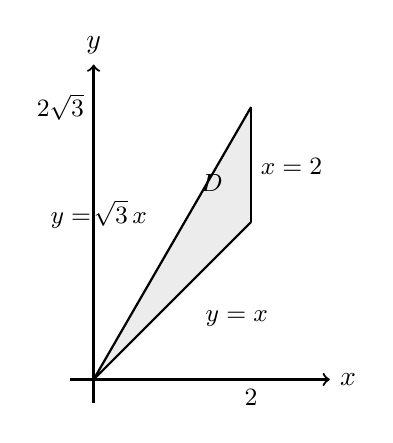
\begin{tikzpicture}
    \draw[thick,->] (-0.3,0) -- (3.0,0) node[right]{$x$};
    \draw[thick,->] (0,-0.3) -- (0,4.0) node[above]{$y$};
    \fill[gray!15] (0,0) -- (2,2) -- (2,3.46) -- cycle;
    \draw[thick] (0,0) -- (2,2);
    \draw[thick] (0,0) -- (2,3.46);
    \draw[thick] (2,2) -- (2,3.46);
    \node[right] at (2,2.7) {\small$x=2$};
    \node[below right] at (1.3,1.0) {\small$y=x$};
    \node[above left] at (0.8,1.8) {\small$y=\!\sqrt{3}\,x$};
    \node at (1.5,2.5) {\small$D$};
    \node[left] at (0,3.46) {\small$2\sqrt{3}$};
    \node[below] at (2,0) {\small$2$};
\end{tikzpicture}
\end{center}

$\theta\in[\pi/4,\,\pi/3]$, \; $r\in[0,\,2\sec\theta]$.
\begin{align*}
    &= \int_{\pi/4}^{\pi/3}\!\int_0^{2\sec\theta}
       r^2\sin\theta\dd{r}\dd{\theta}
    = \int_{\pi/4}^{\pi/3}
       \tfrac{8}{3}\sec^3\!\theta\,\sin\theta\dd{\theta} \\
    &= \frac{8}{3}\!\left[\frac{1}{2\cos^2\theta}\right]_{\pi/4}^{\pi/3}
    = \frac{8}{3}\cdot\frac{1}{2}(4-2)
    = \frac{8}{3}
\end{align*}
\end{example}

\begin{example}
Find $\displaystyle\iint_D x\sqrt{x^2+y^2}\dd{A}$
where $D$ is enclosed by $r^2=\sin 2\theta$ in the first quadrant.

\begin{center}
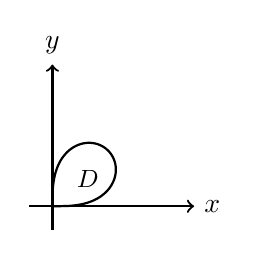
\begin{tikzpicture}
    \draw[thick,->] (-0.3,0) -- (1.8,0) node[right]{$x$};
    \draw[thick,->] (0,-0.3) -- (0,1.8) node[above]{$y$};
    \draw[thick, domain=0:90, samples=100, smooth]
        plot ({sqrt(max(sin(2*\x),0))*cos(\x)},
             {sqrt(max(sin(2*\x),0))*sin(\x)});
    \node at (0.45,0.35) {\small$D$};
\end{tikzpicture}
\end{center}

\begin{align*}
    &= \int_0^{\pi/2}\!\int_0^{\sqrt{\sin 2\theta}}
       r^3\cos\theta\dd{r}\dd{\theta}
    = \int_0^{\pi/2}\tfrac{1}{4}\sin^2\!(2\theta)\,\cos\theta\dd{\theta} \\
    &= \int_0^{\pi/2}\sin^2\!\theta\,\cos^3\!\theta\dd{\theta}
    = \int_0^{\pi/2}\sin^2\!\theta\,(1-\sin^2\!\theta)\cos\theta\dd{\theta} \\
    &= \left[\tfrac{1}{3}\sin^3\!\theta
       -\tfrac{1}{5}\sin^5\!\theta\right]_0^{\pi/2}
    = \frac{2}{15}
\end{align*}
\end{example}

\subsection{Applications of Double Integrals}

Given a region $D$ with density $\rho(x,y)$:

\begin{definition}{Center of Mass}{center-mass}
\[
    \mathbf{c}
    = \frac{1}{\text{mass}}
      \iint_D \rho(x,y)\begin{pmatrix}x\\y\end{pmatrix}\dd{A}
    = \frac{\iint_D \rho\,\mathbf{x}\dd{A}}
           {\iint_D \rho\dd{A}}
\]
\end{definition}

\begin{example}
$\rho(x,y)=1+y$, \; $D$: unit disk $x^2+y^2\le 1$.

\begin{center}
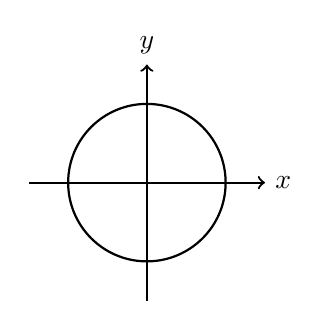
\begin{tikzpicture}
    \draw[thick,->] (-1.5,0) -- (1.5,0) node[right]{$x$};
    \draw[thick,->] (0,-1.5) -- (0,1.5) node[above]{$y$};
    \draw[thick] (0,0) circle (1);
\end{tikzpicture}
\end{center}

\textbf{Mass:}
\[
    \text{Mass}
    = \int_0^{2\pi}\!\int_0^1(1+r\sin\theta)\,r\dd{r}\dd{\theta}
    = \pi
    \qquad\left(\textstyle\int_0^{2\pi}\sin\theta\dd{\theta}=0\right)
\]

\textbf{Center of mass:}
\[
    \text{CoM}
    = \frac{1}{\pi}\iint_D(1+y)
      \begin{pmatrix}x\\y\end{pmatrix}\dd{A}
    = \frac{1}{\pi}
      \begin{pmatrix}
        \iint_D(1+y)\,x\dd{A}\\[4pt]
        \iint_D(1+y)\,y\dd{A}
      \end{pmatrix}
\]

$\bar{x}=0$ by symmetry
($(1+y)\,x$ is odd in $x$ over a symmetric domain).

\begin{align*}
    \bar{y}
    &= \frac{1}{\pi}\int_0^{2\pi}\!\int_0^1
       (1+r\sin\theta)\,r\sin\theta\;r\dd{r}\dd{\theta} \\
    &= \frac{1}{4\pi}\int_0^{2\pi}\sin^2\!\theta\dd{\theta}
    = \frac{1}{4\pi}\cdot\frac{1}{2}
      \int_0^{2\pi}(1-\cos 2\theta)\dd{\theta}
    = \frac{1}{4}
\end{align*}

Center of mass: $\left(0,\;\dfrac{1}{4}\right)$.
\end{example}
